% Options for packages loaded elsewhere
% Options for packages loaded elsewhere
\PassOptionsToPackage{unicode}{hyperref}
\PassOptionsToPackage{hyphens}{url}
\PassOptionsToPackage{dvipsnames,svgnames,x11names}{xcolor}
%
\documentclass[
  british,
  a4paper,
]{article}
\usepackage{xcolor}
\usepackage{amsmath,amssymb}
\setcounter{secnumdepth}{-\maxdimen} % remove section numbering
\usepackage{iftex}
\ifPDFTeX
  \usepackage[T1]{fontenc}
  \usepackage[utf8]{inputenc}
  \usepackage{textcomp} % provide euro and other symbols
\else % if luatex or xetex
  \usepackage{unicode-math} % this also loads fontspec
  \defaultfontfeatures{Scale=MatchLowercase}
  \defaultfontfeatures[\rmfamily]{Ligatures=TeX,Scale=1}
\fi
\usepackage{lmodern}
\ifPDFTeX\else
  % xetex/luatex font selection
\fi
% Use upquote if available, for straight quotes in verbatim environments
\IfFileExists{upquote.sty}{\usepackage{upquote}}{}
\IfFileExists{microtype.sty}{% use microtype if available
  \usepackage[]{microtype}
  \UseMicrotypeSet[protrusion]{basicmath} % disable protrusion for tt fonts
}{}
\makeatletter
\@ifundefined{KOMAClassName}{% if non-KOMA class
  \IfFileExists{parskip.sty}{%
    \usepackage{parskip}
  }{% else
    \setlength{\parindent}{0pt}
    \setlength{\parskip}{6pt plus 2pt minus 1pt}}
}{% if KOMA class
  \KOMAoptions{parskip=half}}
\makeatother
% Make \paragraph and \subparagraph free-standing
\makeatletter
\ifx\paragraph\undefined\else
  \let\oldparagraph\paragraph
  \renewcommand{\paragraph}{
    \@ifstar
      \xxxParagraphStar
      \xxxParagraphNoStar
  }
  \newcommand{\xxxParagraphStar}[1]{\oldparagraph*{#1}\mbox{}}
  \newcommand{\xxxParagraphNoStar}[1]{\oldparagraph{#1}\mbox{}}
\fi
\ifx\subparagraph\undefined\else
  \let\oldsubparagraph\subparagraph
  \renewcommand{\subparagraph}{
    \@ifstar
      \xxxSubParagraphStar
      \xxxSubParagraphNoStar
  }
  \newcommand{\xxxSubParagraphStar}[1]{\oldsubparagraph*{#1}\mbox{}}
  \newcommand{\xxxSubParagraphNoStar}[1]{\oldsubparagraph{#1}\mbox{}}
\fi
\makeatother


\usepackage{longtable,booktabs,array}
\newcounter{none} % for unnumbered tables
\usepackage{calc} % for calculating minipage widths
% Correct order of tables after \paragraph or \subparagraph
\usepackage{etoolbox}
\makeatletter
\patchcmd\longtable{\par}{\if@noskipsec\mbox{}\fi\par}{}{}
\makeatother
% Allow footnotes in longtable head/foot
\IfFileExists{footnotehyper.sty}{\usepackage{footnotehyper}}{\usepackage{footnote}}
\makesavenoteenv{longtable}
\usepackage{graphicx}
\makeatletter
\newsavebox\pandoc@box
\newcommand*\pandocbounded[1]{% scales image to fit in text height/width
  \sbox\pandoc@box{#1}%
  \Gscale@div\@tempa{\textheight}{\dimexpr\ht\pandoc@box+\dp\pandoc@box\relax}%
  \Gscale@div\@tempb{\linewidth}{\wd\pandoc@box}%
  \ifdim\@tempb\p@<\@tempa\p@\let\@tempa\@tempb\fi% select the smaller of both
  \ifdim\@tempa\p@<\p@\scalebox{\@tempa}{\usebox\pandoc@box}%
  \else\usebox{\pandoc@box}%
  \fi%
}
% Set default figure placement to htbp
\def\fps@figure{htbp}
\makeatother



\ifLuaTeX
\usepackage[bidi=basic,shorthands=off]{babel}
\else
\usepackage[bidi=default,shorthands=off]{babel}
\fi
\ifLuaTeX
  \usepackage{selnolig} % disable illegal ligatures
\fi


\setlength{\emergencystretch}{3em} % prevent overfull lines

\providecommand{\tightlist}{%
  \setlength{\itemsep}{0pt}\setlength{\parskip}{0pt}}



 


\makeatletter
\@ifpackageloaded{tcolorbox}{}{\usepackage[skins,breakable]{tcolorbox}}
\@ifpackageloaded{fontawesome5}{}{\usepackage{fontawesome5}}
\definecolor{quarto-callout-color}{HTML}{909090}
\definecolor{quarto-callout-note-color}{HTML}{0758E5}
\definecolor{quarto-callout-important-color}{HTML}{CC1914}
\definecolor{quarto-callout-warning-color}{HTML}{EB9113}
\definecolor{quarto-callout-tip-color}{HTML}{00A047}
\definecolor{quarto-callout-caution-color}{HTML}{FC5300}
\definecolor{quarto-callout-color-frame}{HTML}{acacac}
\definecolor{quarto-callout-note-color-frame}{HTML}{4582ec}
\definecolor{quarto-callout-important-color-frame}{HTML}{d9534f}
\definecolor{quarto-callout-warning-color-frame}{HTML}{f0ad4e}
\definecolor{quarto-callout-tip-color-frame}{HTML}{02b875}
\definecolor{quarto-callout-caution-color-frame}{HTML}{fd7e14}
\makeatother
\makeatletter
\@ifpackageloaded{caption}{}{\usepackage{caption}}
\AtBeginDocument{%
\ifdefined\contentsname
  \renewcommand*\contentsname{Table of contents}
\else
  \newcommand\contentsname{Table of contents}
\fi
\ifdefined\listfigurename
  \renewcommand*\listfigurename{List of Figures}
\else
  \newcommand\listfigurename{List of Figures}
\fi
\ifdefined\listtablename
  \renewcommand*\listtablename{List of Tables}
\else
  \newcommand\listtablename{List of Tables}
\fi
\ifdefined\figurename
  \renewcommand*\figurename{Figure}
\else
  \newcommand\figurename{Figure}
\fi
\ifdefined\tablename
  \renewcommand*\tablename{Table}
\else
  \newcommand\tablename{Table}
\fi
}
\@ifpackageloaded{float}{}{\usepackage{float}}
\floatstyle{ruled}
\@ifundefined{c@chapter}{\newfloat{codelisting}{h}{lop}}{\newfloat{codelisting}{h}{lop}[chapter]}
\floatname{codelisting}{Listing}
\newcommand*\listoflistings{\listof{codelisting}{List of Listings}}
\makeatother
\makeatletter
\makeatother
\makeatletter
\@ifpackageloaded{caption}{}{\usepackage{caption}}
\@ifpackageloaded{subcaption}{}{\usepackage{subcaption}}
\makeatother
\usepackage{bookmark}
\IfFileExists{xurl.sty}{\usepackage{xurl}}{} % add URL line breaks if available
\urlstyle{same}
% fallback for those not using the hyperref driver hyperxmp:
\makeatletter
\@ifundefined{xmpquote}{\newcommand{\xmpquote}[1]{#1}}{}
\makeatother
\hypersetup{
  pdftitle={A cross-country macro panel and what global shocks do to small open economies},
  pdfauthor={Carlos Galindo},
  pdflang={en-GB},
  colorlinks=true,
  linkcolor={blue},
  filecolor={Maroon},
  citecolor={Blue},
  urlcolor={Blue},
  pdfcreator={LaTeX via pandoc}}


\title{A cross-country macro panel and what global shocks do to small
open economies}
\usepackage{etoolbox}
\makeatletter
\providecommand{\subtitle}[1]{% add subtitle to \maketitle
  \apptocmd{\@title}{\par {\large #1 \par}}{}{}
}
\makeatother
\subtitle{An automated monthly and quarterly panel for five small open
economies, organised around global shocks, uncertainty and financial
vulnerability}
\author{Carlos Galindo}
\date{}
\begin{document}
\maketitle


\begin{tcolorbox}[enhanced jigsaw, arc=.35mm, bottomrule=.15mm, breakable, colback=white, colframe=quarto-callout-note-color-frame, left=2mm, leftrule=.75mm, opacityback=0, rightrule=.15mm, toprule=.15mm]

\vspace{-3mm}\textbf{At a glance}\vspace{3mm}

\begin{itemize}
\tightlist
\item
  \textbf{Question.} What do global shocks, macroeconomic uncertainty
  and financial-sector fragility do to small open economies, and can one
  harmonised data panel answer it routinely?
\item
  \textbf{Approach.} An automated monthly and quarterly panel for five
  economies, built from international official sources under strict
  frequency and aggregation rules, plus early-warning indicators for 63
  jurisdictions.
\item
  \textbf{Finding.} One harmonised panel now serves monthly and
  quarterly analysis of five economies, with debt-service and credit-gap
  early-warning indicators for 63 jurisdictions. Its first use, a
  dynamic panel of industrial output, found global market volatility the
  one channel that survives every specification and no robust direct
  effect of domestic policy rates.
\item
  \textbf{Why it matters.} The panel turns a one-off analysis into a
  routine diagnostic that can be refreshed as new data arrive.
\end{itemize}

\end{tcolorbox}

\subsection{The question}\label{the-question}

Small open economies are price-takers in global markets. Poland,
Hungary, the Czech Republic, South Africa and Israel differ in size,
monetary regime and exposure, yet their output, exchange rates and
funding costs often move together when global conditions change. A macro
analyst covering them needs three things at once: a comparable record of
what is happening at home, a consistent measure of the global
environment, and an early read on where the financial system is
stretched.

The obvious approach, a country-by-country spreadsheet refreshed by
hand, falls short in three ways. Definitions drift between countries and
over time. Mixing monthly and quarterly series quietly invents data. And
nothing is repeatable, so a conclusion cannot be checked a month later
when the numbers have been revised.

This project builds the panel so that those problems are handled by
design, and then uses it to ask what the global environment does to
domestic activity.

\subsection{Approach}\label{approach}

\textbf{Data.} The panel covers five small open economies at monthly and
quarterly frequency from 1999 onward. It draws on international official
sources and comprises 182 series: 60 global series (market volatility,
commodities, US rates and activity, uncertainty and geopolitical-risk
indices, credit and sentiment measures) and 122 country-specific series
covering prices, output, labour markets, policy rates, exchange rates,
external accounts, fiscal positions and financial stability. Global
series are fetched once and attached to every country, so every economy
faces an identical global backdrop.

\textbf{Design rules.} Three rules do most of the work.

\begin{itemize}
\tightlist
\item
  The monthly panel contains monthly series only. Quarterly or annual
  series are never forward-filled into months; they live in the
  quarterly panel instead.
\item
  When series are aggregated up to quarters, the rule follows the
  economic type: flows are summed, stocks are averaged or taken at
  period end, and rates are averaged.
\item
  Seasonally adjusted and unadjusted series are not mixed, units and
  transformations are audited, and every series carries its source and
  revision history so a later refresh can be compared with an earlier
  one.
\end{itemize}

\textbf{Diagnostics framework.} The panel is organised around three
blocks: global shocks, macroeconomic uncertainty, and financial-sector
vulnerability. For the last, a wider early-warning dataset of
debt-service ratios and credit-to-GDP gaps covers 63 jurisdictions, with
histories reaching back to the 1920s for some. The five-economy panel
inherits the same indicators.

\textbf{Estimation.} Industrial output growth is modelled as a dynamic
panel: its own lag, the policy rate, inflation, the change in the
sovereign spread, oil prices, and a market volatility index. Estimators
include pooled and fixed-effects least squares, fixed effects with
standard errors clustered by time (so that contemporaneous cross-country
correlation is respected), and two instrumental-variable estimators in
first differences. The panel is balanced with five countries and about
326 months, from January 1999 to February 2026, so fixed-effects bias
from the lagged dependent variable is small.

\textbf{Checking.} Results were compared across estimators and
re-estimated after a data correction to one country's price series.
Where the original dynamic-panel estimation used a very large instrument
set relative to five countries, it was replaced by a parsimonious one
and the test of instrument validity re-run.

\subsection{What the work shows}\label{what-the-work-shows}

\textbf{Persistence dominates.} Industrial growth carries strong
inertia: the own-lag coefficient is about 0.84 in the fixed-effects
model, implying a half-life of roughly four months. The ordering across
estimators is what theory predicts, with pooled estimates highest and
the instrumental-variable estimates lower, at about 0.67 to 0.70.

\begin{figure}

\centering{

\pandocbounded{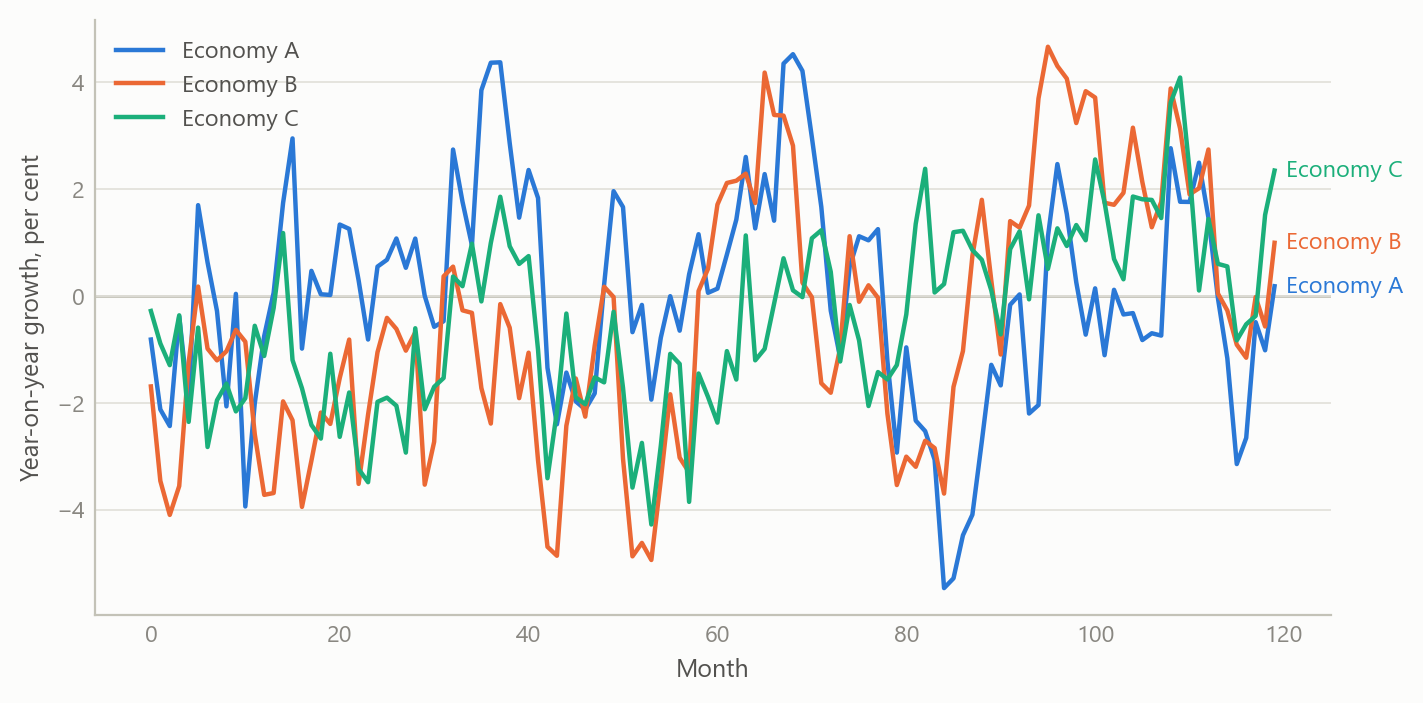
\includegraphics[keepaspectratio]{index_files/figure-latex/fig-persistence-output-1.png}}

}

\caption{\label{fig-persistence}Industrial output growth in five small
open economies: a common global factor plus strong persistence
(simulated data).}

\end{figure}%

\textbf{Global risk appetite is the one robust channel.} A rise in
market-implied volatility lowers industrial growth contemporaneously by
about 0.09 to 0.10 percentage points per index point, and the result
holds in both the fixed-effects and instrumental-variable
specifications. Because output is persistent, the cumulative cost of a
one-off 20-point volatility spike is roughly 9.7 percentage points of
growth, spread over several months, with an impact effect near 1.9
points.

\begin{figure}

\centering{

\pandocbounded{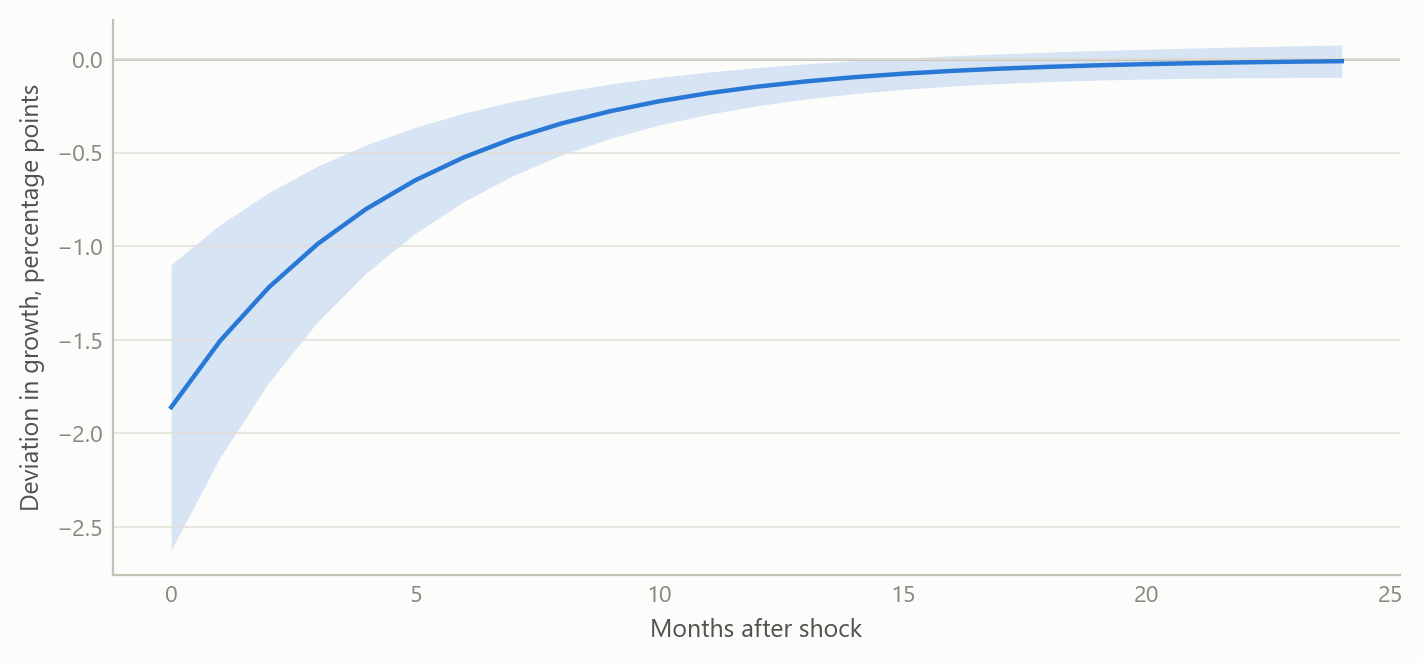
\includegraphics[keepaspectratio]{index_files/figure-latex/fig-shock-output-1.png}}

}

\caption{\label{fig-shock}Illustrative response of industrial growth to
a one-off 20-point rise in market volatility, with an uncertainty band
(simulated data).}

\end{figure}%

\textbf{Domestic policy rates show no robust direct effect.} The
policy-rate coefficient is statistically indistinguishable from zero in
every specification. A significant negative result that appeared under
the earlier, over-instrumented estimation disappeared once the
instrument set was made credible, and the test of instrument validity
then no longer rejected. The most plausible reading is two offsetting
forces: tightening dampens output, while central banks tighten when the
economy is strong.

\textbf{Oil and spreads.} Oil prices are insignificant in levels but
positive and significant in first differences, which fits oil acting as
a proxy for global demand rather than as a pure cost shock. The change
in the sovereign spread has no contemporaneous effect. That does not
make sovereign risk irrelevant: it more plausibly works through longer
lags, spread levels, or thresholds that only extreme episodes cross.

\begin{longtable}[]{@{}
  >{\raggedright\arraybackslash}p{(\linewidth - 12\tabcolsep) * \real{0.1111}}
  >{\raggedleft\arraybackslash}p{(\linewidth - 12\tabcolsep) * \real{0.1481}}
  >{\raggedleft\arraybackslash}p{(\linewidth - 12\tabcolsep) * \real{0.1481}}
  >{\raggedleft\arraybackslash}p{(\linewidth - 12\tabcolsep) * \real{0.1481}}
  >{\raggedleft\arraybackslash}p{(\linewidth - 12\tabcolsep) * \real{0.1481}}
  >{\raggedleft\arraybackslash}p{(\linewidth - 12\tabcolsep) * \real{0.1481}}
  >{\raggedleft\arraybackslash}p{(\linewidth - 12\tabcolsep) * \real{0.1481}}@{}}
\caption{Dynamic-panel estimates for industrial output growth (year on
year, per cent), five economies, monthly, 1999 to 2026. Standard errors
in parentheses; the robust column clusters by month; the two
instrumental-variable estimators are in first differences. ***
p\textless0.01, ** p\textless0.05, * p\textless0.10. In the
monetary-channel specification the volatility coefficient is −0.093
(0.023) under fixed effects with month-clustered errors and −0.103
(0.028) under the first-difference instrumental-variable estimator, both
p\textless0.01. Source: public macroeconomic and market series; the
author's estimates.}\label{tbl-panel-estimates}\tabularnewline
\toprule\noalign{}
\begin{minipage}[b]{\linewidth}\raggedright
\end{minipage} & \begin{minipage}[b]{\linewidth}\raggedleft
Pooled OLS
\end{minipage} & \begin{minipage}[b]{\linewidth}\raggedleft
Fixed effects
\end{minipage} & \begin{minipage}[b]{\linewidth}\raggedleft
Fixed effects, robust
\end{minipage} & \begin{minipage}[b]{\linewidth}\raggedleft
Fixed effects, GLS
\end{minipage} & \begin{minipage}[b]{\linewidth}\raggedleft
GMM (Arellano-Bond)
\end{minipage} & \begin{minipage}[b]{\linewidth}\raggedleft
IV (Anderson-Hsiao)
\end{minipage} \\
\midrule\noalign{}
\endfirsthead
\toprule\noalign{}
\begin{minipage}[b]{\linewidth}\raggedright
\end{minipage} & \begin{minipage}[b]{\linewidth}\raggedleft
Pooled OLS
\end{minipage} & \begin{minipage}[b]{\linewidth}\raggedleft
Fixed effects
\end{minipage} & \begin{minipage}[b]{\linewidth}\raggedleft
Fixed effects, robust
\end{minipage} & \begin{minipage}[b]{\linewidth}\raggedleft
Fixed effects, GLS
\end{minipage} & \begin{minipage}[b]{\linewidth}\raggedleft
GMM (Arellano-Bond)
\end{minipage} & \begin{minipage}[b]{\linewidth}\raggedleft
IV (Anderson-Hsiao)
\end{minipage} \\
\midrule\noalign{}
\endhead
\bottomrule\noalign{}
\endlastfoot
Lagged output growth & 0.849*** & 0.842*** & 0.842*** & 0.845*** &
0.673*** & 0.702*** \\
& (0.014) & (0.014) & (0.029) & (0.014) & (0.142) & (0.124) \\
Policy rate & −0.017 & −0.014 & −0.014 & −0.020 & 0.190 & 0.231 \\
& (0.034) & (0.040) & (0.076) & (0.040) & (0.341) & (0.376) \\
Inflation & −0.059* & −0.065* & −0.065 & −0.064* & −0.232 & −0.270 \\
& (0.035) & (0.036) & (0.050) & (0.035) & (0.209) & (0.226) \\
Change in sovereign spread & −0.023 & −0.003 & −0.003 & 0.013 & 0.153 &
0.125 \\
& (0.293) & (0.293) & (0.440) & (0.299) & (0.333) & (0.323) \\
Oil price & 0.002 & 0.002 & 0.002 & 0.002 & 0.050** & 0.051** \\
& (0.004) & (0.004) & (0.006) & (0.004) & (0.023) & (0.021) \\
Observations & 1,442 & 1,442 & 1,442 & 1,442 & 1,431 & 1,434 \\
\end{longtable}

\textbf{Financial vulnerability.} The wider early-warning dataset
records debt-service ratios and credit-to-GDP gaps for 63 jurisdictions.
The figure below shows the kind of screen the framework supports:
jurisdictions with a high debt-service burden and a positive credit gap
are flagged for closer attention.

\begin{figure}

\centering{

\pandocbounded{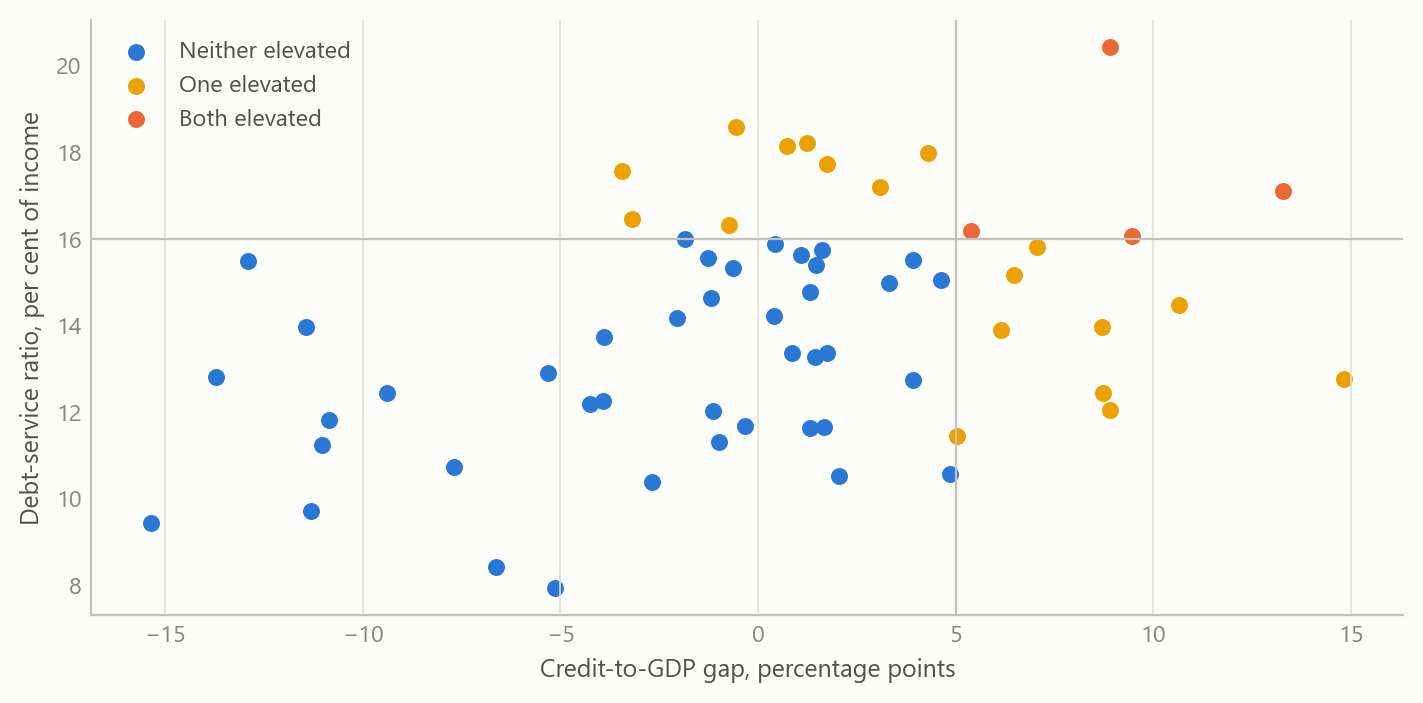
\includegraphics[keepaspectratio]{index_files/figure-latex/fig-ewi-output-1.png}}

}

\caption{\label{fig-ewi}Early-warning screen for 63 jurisdictions:
credit gap against debt-service ratio, flagged where both are elevated
(simulated data).}

\end{figure}%

\subsection{Insights}\label{insights}

\begin{enumerate}
\def\labelenumi{\arabic{enumi}.}
\tightlist
\item
  \textbf{Build the panel before the model.} Most of the value sat in
  the harmonised, rule-governed panel. Once definitions, frequencies and
  aggregation are fixed, each new question becomes a short exercise
  rather than a new data project.
\item
  \textbf{Respect frequency.} Refusing to forward-fill quarterly data
  into months costs some coverage but avoids spurious precision.
  Separate monthly and quarterly panels keep the claim honest.
\item
  \textbf{Instrument sets must suit the sample.} With five countries and
  many months, a large dynamic instrument set produced a pathological
  test statistic and a spurious policy effect. A parsimonious set gave a
  credible result. This lesson transfers to any small-N dynamic panel.
\item
  \textbf{A data correction can change conclusions.} Fixing one
  country's price series changed the size and significance of several
  coefficients, which is why every series carries its provenance.
\item
  \textbf{Some gaps are real.} For some countries, series such as
  quarterly government debt, core inflation or debt-service ratios have
  no public source. Recording those gaps explicitly is better than
  filling them with proxies.
\end{enumerate}

\subsection{Limits and next steps}\label{limits-and-next-steps}

The panel has only five economies, so the results describe a small
group, not emerging markets in general. Estimates are contemporaneous
and linear; they do not capture thresholds or longer credit lags, and
the volatility effect may partly reflect common global demand. The
activity model uses one output measure and should be extended to
labour-market and external-account outcomes. The downstream step,
turning the diagnostics into regular written macro briefs, has been
designed but not built. The early-warning screen needs a validated
threshold and an out-of-sample test before any ranking is used.

\subsection{About the evidence}\label{about-the-evidence}

The panel and the dynamic-panel estimates are the project's own work
during a career break, from late 2025 to early 2026, built with AI
assistance under my direction as systems architect. The text and the
table report real results from that work; the table was re-fitted from
the stored panel, which reproduces the reported estimates exactly. The
figures here are simulated to share its structure (five units, monthly
frequency, 63 jurisdictions) and are not the project's estimates.

Figures and tables marked \emph{simulated} are generated from simulated
data built to share the structure of the analysis (its variables,
horizons and frequencies). They show how the method works and what its
output looks like; they are not the project's results. Results stated in
the text are the project's own. Methods are described at the level of a
methods section. Code and data pipelines are not reproduced here.




\end{document}
